\documentclass[10pt]{article}

\usepackage{fancyhdr}
\usepackage[includeheadfoot,left=1in, right=0.5in, top=0.5in, bottom=0.5in]{geometry}
\usepackage{lastpage}
\usepackage{extramarks}
\usepackage[usenames,dvipsnames]{color}
\usepackage{graphicx}
\usepackage{listings}
\usepackage{courier}
\usepackage{tikz}
\usepackage{color}
\usepackage{float}
\usepackage{url}
\usepackage{subfigure}
\usepackage{varwidth}
\usepackage{caption}
\usepackage{multirow}
\usepackage[pdfborder={0 0 0}]{hyperref}
\usepackage[compact,small]{titlesec}
\usepackage{microtype}
\usepackage{verbatim}
\usepackage{booktabs}
\usepackage{indentfirst}
\usepackage{pbox}
\usepackage{dcolumn}

\parskip = 0.5\baselineskip
\setlength{\belowcaptionskip}{-\baselineskip}

\captionsetup{font=scriptsize}
\captionsetup{labelfont=bf}

\pagestyle{fancy}
\rhead{Max Thrun}
\lhead{EECE6086 - HW 1}
\rfoot{Page\ \thepage\ of \protect\pageref{LastPage}}
\cfoot{}
\renewcommand\headrulewidth{0.4pt}
\renewcommand\footrulewidth{0.4pt}

% make verbatim text small
\makeatletter
\g@addto@macro\@verbatim\small
\makeatother

\setlength\parindent{0pt} % Removes all indentation from paragraphs

\definecolor{sh_comment}{rgb}{0.12, 0.38, 0.18 } %adjusted, in Eclipse: {0.25, 0.42, 0.30 } = #3F6A4D
\definecolor{sh_keyword}{rgb}{0.37, 0.08, 0.25}  % #5F1441
\definecolor{sh_string}{rgb}{0.06, 0.10, 0.98} % #101AF9

\lstset{
    language=c++,
    xleftmargin=.25in,
    xrightmargin=.25in,
    numbers=left,
    numberstyle=\tiny,
    frame=tb,
    showstringspaces=false,
    captionpos=b,
    stringstyle=\color{sh_string},
    keywordstyle = \color{sh_keyword}\bfseries,
    commentstyle=\color{sh_comment}\itshape,
    basicstyle=\footnotesize\sffamily,
    %numbersep=-5pt,
    belowskip=\baselineskip,
    aboveskip=\baselineskip
}

\let\oldtabular\tabular
\renewcommand{\tabular}{\footnotesize\oldtabular}

\title{
    \vspace{2in}
    \textmd{\textbf{EECE6086 - HW 1}}\\
    \vspace{4in}
}
\author{\textbf{Max Thrun}}

\begin{document}
\maketitle
\newpage
\section{Objective}

The objective of this assignment was to implement the Kernighan---Lin graph
partitioning algorithm and attempt to achieve the smallest cutsize in the
shortest amount of time.

\section{Implementation Details}

My implementation of the KL algorithm is fairly standard with the exception of
how nodes are selected to be swapped. Traditionally, nodes of each group are
exhaustively combined in order to see which pair results in the greatest
cutsize reduction. After testing the original algorithm and seeing how
incredibly slow this method is I have decided that instead of testing every
combination it is sufficient to just select the two most costly nodes from each
group. While there are definitely some cases where this method is unable to
reach to exact optimal cutsize the speed boost gained by avoiding the
exhaustive search is enormous.

My first implementation attempt was written in Python (see \texttt{parprog.py})
in order to prove I understood the algorithm and that it was working correctly.
This also helped serve as a baseline to check my C++ implementation against.
Unsurprisingly, the Python implementation was incredibly slow which made it
virtually unusable.  I then reimplemented it in C++ using all the same data
structures (maps, sets, etc...).  While this implementation was significantly
faster I found after profiling it that it spent the majority of its execution
time in the standard library dealing with these complex data structures. I then
iteratively went through the process of converting my structures into something
simpler (basically flat arrays) and re-profiling my code.  As it stands now all
my data structures are just flat integer arrays with the exception of my sparse
connection matrix which is a flat array of type \texttt{std::unordered\_set}. I
decided to use a set to hold the connections for each cell for two main
reasons. Firstly, I needed a dynamically sized array and secondly I needed to
be able to quickly see if a value is contained within the array. These
requirements leave \texttt{std::unordered\_set} as the only logical datatype.
The choice of \texttt{std::unordered\_set} over \texttt{std:set} was that the
unordered version provides a faster lookup time as it is implemented with a
hashtable.

I also implemented an optional `cheat' mode which only continues searching for
a longer swap subset so long as the current swap cost is positive. As we'll see
later this leads to a significant decrease in execution time at the cost of
slightly higher cutsizes in some cases.

A very high level psuedo code overview is shown below.
\begin{lstlisting}[caption=Implementation Psuedo Code]
read in connection pairs
split nodes into two even groups
while 1
    loop through all connections and compute cost
    for k in (num_cells / 2)
        loop through all cells
            if cell is marked skip it
            if cell is in group A
                check if it is new maximum of group A
            if cell is in group B
                check if it is new maximum of group B
        if maximum of group A is connected to maximum of group B
            cost = cost_a + cost_b - 2
        else
            cost = cost_a + cost_b
        cost_sum += cost
        if cost_sum > cost_max
            store current cost_sum as cost_max
            save this k value (k_max)
        record what nodes we swapped
        mark them as swapped
        update the costs of effected nodes
    if cost_max <= 0
        exit and print results
    else
        exchange up to k_max cells
\end{lstlisting}

\newpage
\section{Usage}

Building is accomplished via a Makefile which generates an executable named
\texttt{parprog}.  Additional build options are shown below

\begin{lstlisting}[language=bash]
$ make              # regular build
$ make cheat        # builds with the swap subset cheat
$ make benchmarks   # runs all the benchmarks in the BM directory
\end{lstlisting}

The program accepts input via \texttt{stdin} and will write the final output to
\texttt{stdout}.  These can be redirected from and to a file respectively.
Debugging/Status messages are written to \texttt{stderr}. The first line of the
output file is the achieved cutsize. The next two lines are the A and B groups
respectively.  The final line is the CPU execution time in seconds.

\begin{lstlisting}[language=bash]
$ ./parprog < BM/B1 > R1
Num verts: 50
Num edges: 150
========== Iteration 1 ==========
k_max: 13 cost_max: 41
Elapsed time: 0.000000 seconds
========== Iteration 2 ==========
k_max: 1 cost_max: 8
Elapsed time: 0.000000 seconds
========== Iteration 3 ==========
k_max: 0 cost_max: 0
Done
$ cat R1 
15
2 3 6 8 9 11 13 14 16 21 22 23 25 26 28 29 33 34 36 37 38 41 42 45 50 
1 4 5 7 10 12 15 17 18 19 20 24 27 30 31 32 35 39 40 43 44 46 47 48 49 
0.000000
\end{lstlisting}

\newpage
\section{Results}

All benchmarks were compiled and run with the following compiler and CPU

\begin{verbatim}
g++-4.8.2 -Ofast -std=c++0x -march=native -Wall -flto -funroll-loops
Intel i7 920 @ 2.67Ghz
\end{verbatim}

The table below summerizes the results for the given benchmark files.

\newcommand{\specialcell}[2][c]{\textbf{\begin{tabular}[#1]{@{}c@{}}#2\end{tabular}}}
%\newcolumntype{d}{D{.}{.}{3.3} }
\newcolumntype{d}{D{+}{\,\pm\,}{3 ,3 }}
\newcolumntype{e}{D{+}{\,\pm\,}{4 ,2 }}
\begin{table}[H]
    \centering
    \begin{tabular}{cllcccc}
        \toprule
        \textbf{Name} & \textbf{\# Cells} & \textbf{\# Nets} & \specialcell{Given\\Cutsize} & \specialcell{Achieved\\Cutsize} & \specialcell{Execution\\Time} & \specialcell{Memory\\Usage}\\
        \midrule
        B1 & 50     & 150     & 15   & 15    & \phantom{0}0.00s & \phantom{00}1.068 MB\\
        B2 & 500    & 3500    & -    & 346   & \phantom{0}0.00s & \phantom{00}1.328 MB\\
        B3 & 4500   & 27000   & 401  & 405   & \phantom{0}0.16s & \phantom{00}3.708 MB\\
        B4 & 10000  & 150000  & -    & 916   & \phantom{0}0.96s & \phantom{0}14.532 MB\\
        B5 & 25000  & 500000  & 4346 & 4346  & \phantom{0}5.62s & \phantom{0}45.680 MB\\
        B6 & 45000  & 450000  & -    & 2624  &           15.57s & \phantom{0}42.248 MB\\
        B7 & 50000  & 500000  & -    & 4274  &           19.16s & \phantom{0}46.740 MB\\
        B8 & 100000 & 5000000 & -    & 28486 &           87.62s & 437.000 MB\\
        \bottomrule
    \end{tabular}
    \caption{Final Benchmark Results}
\end{table}

The table below shows the orinal benchmarks versus the benchmarks achieved
using the cheaty method described earlier. We can see that exiting the swap
subset search as soon as we see a negative cost allows us to achieve at least a
3x increase in speed. Interestingly, for all the given benchmarks we achieved
the same cutsizes with the exception of B3.
\begin{table}[H]
    \centering
    \begin{tabular}{c|cc|cc|c}
        \toprule
        \textbf{Name} & \specialcell{Achieved\\Cutsize} & \specialcell{Execution\\Time} & \specialcell{Achieved\\Cutsize} & \specialcell{Execution\\Time} & \textbf{Speedup}\\
        \midrule
        B1 & 15    & \phantom{0}0.00s & 15    & \phantom{0}0.00s & - \\
        B2 & 346   & \phantom{0}0.00s & 346   & \phantom{0}0.00s & - \\
        B3 & 405   & \phantom{0}0.16s & 406   & \phantom{0}0.05s & 3.20x \\
        B4 & 916   & \phantom{0}0.96s & 916   & \phantom{0}0.32s & 3.00x \\
        B5 & 4346  & \phantom{0}5.62s & 4346  & \phantom{0}1.64s & 3.42x \\
        B6 & 2624  &           15.57s & 2624  & \phantom{0}3.32s & 4.68x \\
        B7 & 4274  &           19.16s & 4274  & \phantom{0}3.80s & 5.04x \\
        B8 & 28486 &           87.62s & 28486 &           22.40s & 3.91x \\
        \bottomrule
    \end{tabular}
    \caption{Cheaty Benchmark Results}
\end{table}

Just checking against the 8 given benchmarks was not enough to determine if the
cheaty method was good enough to become the default. To test it I generated
1000 random netlists with up to 25,000 cells and 1,250,000 nets. I then
calculated the percent increase in cutsize of the cheaty method over the original
method. I found that on average the cheaty method increased the cutsize by
around 20\%. I felt that this was too high for the cheaty method to become the
default so I left it as a build option.
\begin{figure}[H]
    \centering
    \begin{minipage}{.5\textwidth}
        \centering
        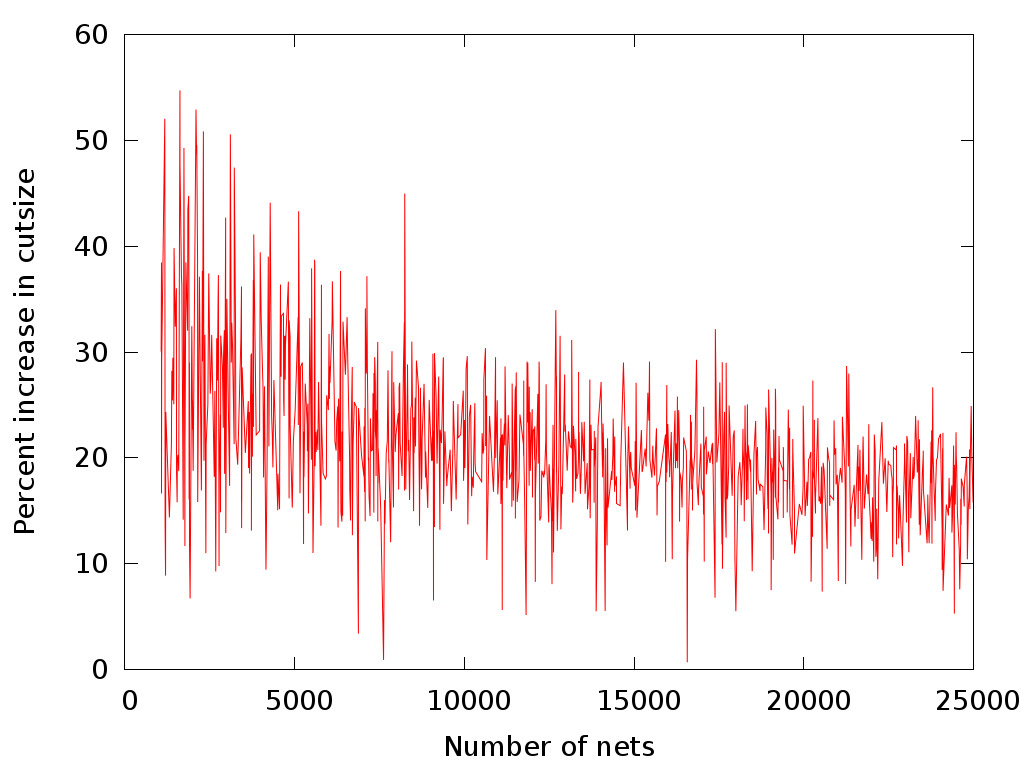
\includegraphics[width=0.8\linewidth]{../tests/cheat_vs_original.png}
    \end{minipage}%
    \begin{minipage}{.5\textwidth}
        \centering
        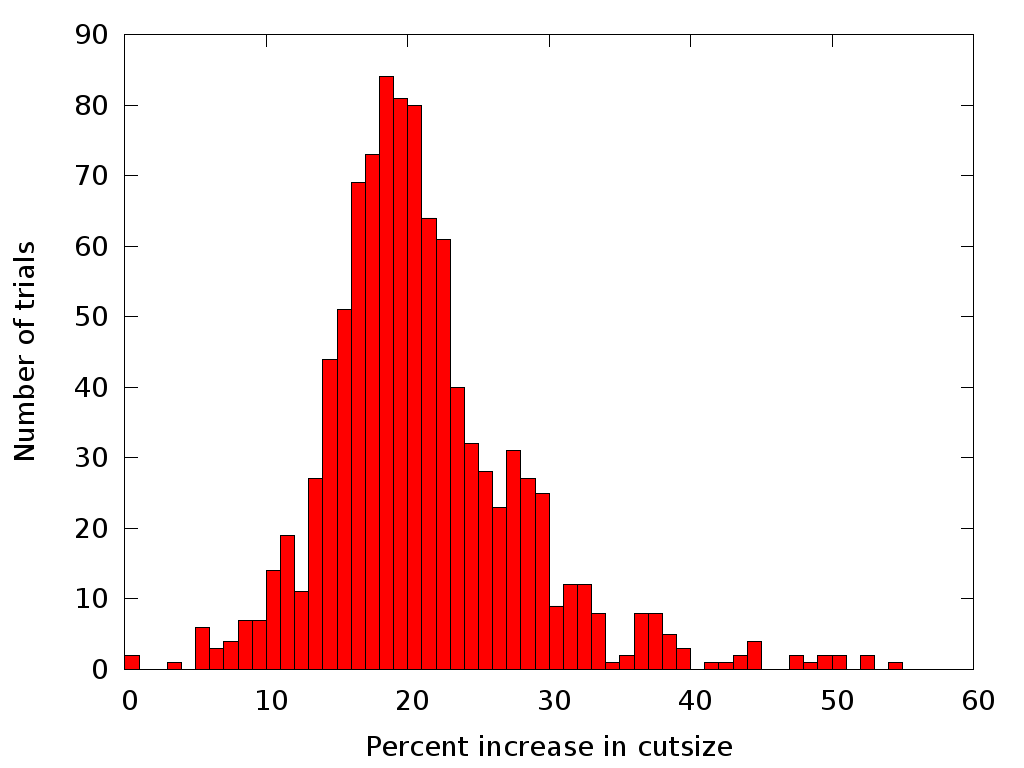
\includegraphics[width=0.8\linewidth]{../tests/cheat_vs_original_hist.png}
    \end{minipage}
    \caption{Percent increase in cutsize using subset search cheat}
\end{figure}

\newpage
\section{Performance Trends}

In order to get an overall idea about the performance of my implementation I
measured the execution time of the 1000 randomly generated netlists.
Specifically, I wanted to see how the number of cells and nets each effected
the execution time.  The two line graphs below show the execution time vs the
number of cells and nets. Without figuring out the actual complexity of our
algorithm we can only guess the type of curve that best fits our data. After
fitting both linear and exponential curves I found the linear curve to be the
best fit. This conclusion may be deceiving given that I am only going up to 25,000
cells. Plugging in 100,000 cells, which is the number of cells in B8, we find
that our trendline predicts an execution time of 90 seconds. This is very close
to the actual time of 87 seconds which gives us confidence that this trendline
is true at least up to 100,000 cells.  In reality the total execution time is
really dependant on both the number of cells \textbf{and} the number of nets
which is easy to visualize in the heatmap shown below. To truly form an
accurate equation we would need to fit a 3D curve which I did not attempt.

\begin{figure}[H]
    \centering
    \begin{minipage}{.5\textwidth}
        \centering
        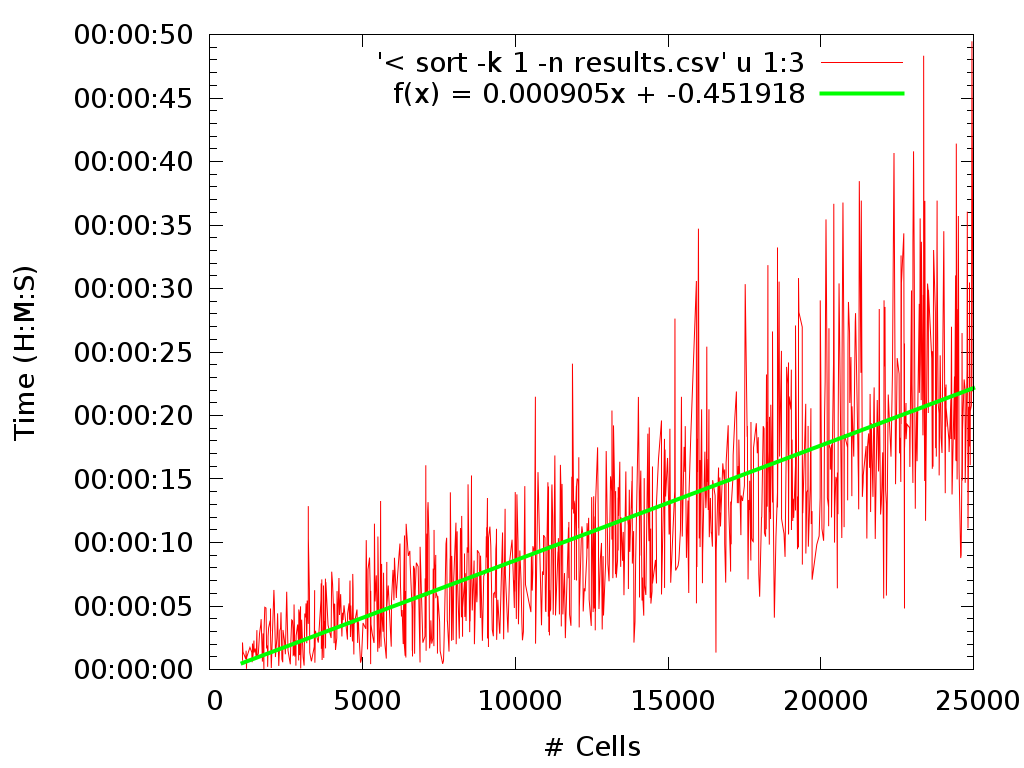
\includegraphics[width=0.8\linewidth]{../tests/result_cells.png}
        \captionof{figure}{Time vs \#Cells}
        \label{fig:test1}
    \end{minipage}%
    \begin{minipage}{.5\textwidth}
        \centering
        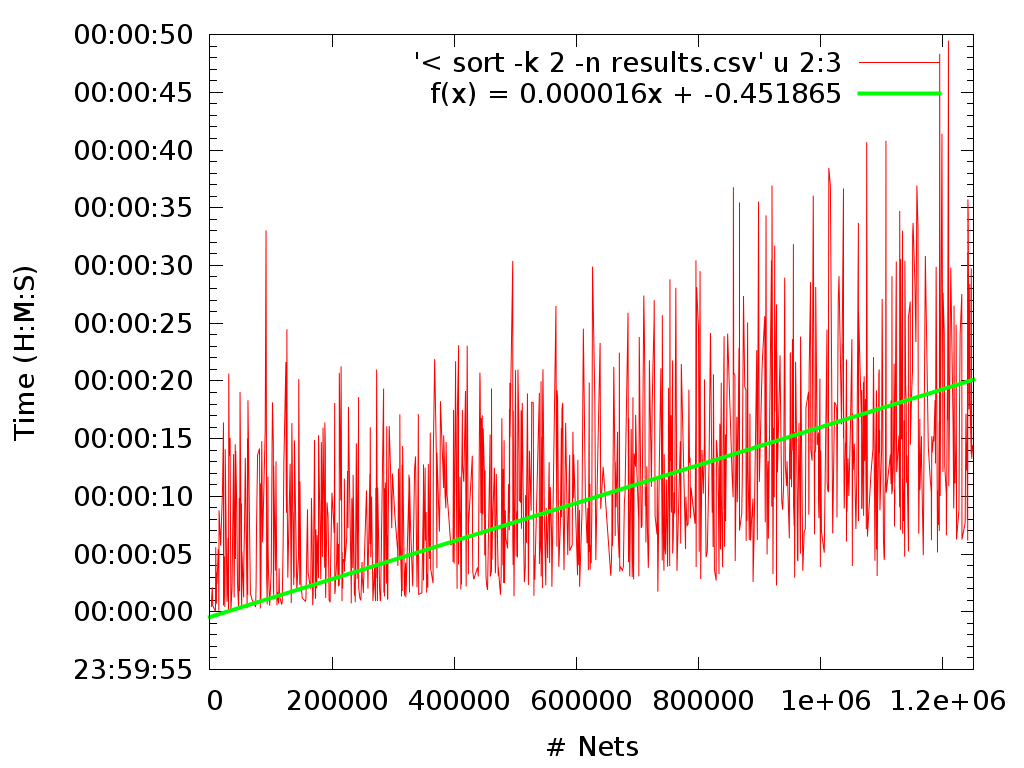
\includegraphics[width=0.8\linewidth]{../tests/result_nets.png}
        \captionof{figure}{Time vs \#Nets}
        \label{fig:test2}
    \end{minipage}
\end{figure}

\begin{figure}[H]
    \centering
    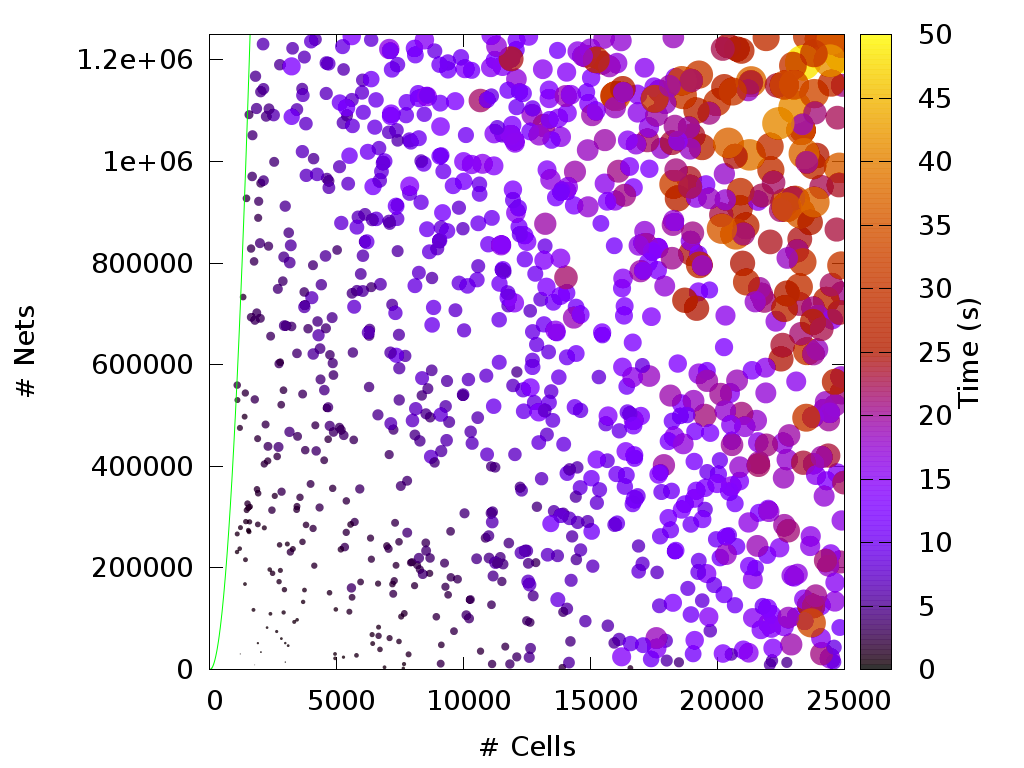
\includegraphics[width=0.8\linewidth]{../tests/result_heatmap.png}
    \caption{Time vs \#Cells \& \#Nets (size of circle proportional to square root of time)}
\end{figure}



\end{document}
